% !TEX root = ../thesis.tex

\chapter{Applications}
\label{chap:applications}

\cleanchapterquote{It is useless to dream of revolution through content, useless to dream of a revelation through form.}{Jean Baudrillard}{(Simulacra and Simulation)}


% ------------------------------------------------------------------------------

In Chapter~\ref{chap:system} we introduced \citeauthor{Gatys2015B}'s Neural Style algorithm for style transfer on images, showing how the knowledge acquired by pre-trained deep neural networks and the concepts behind generative models can be used to solve long-standing problems like the separation of style and content in images.

In this chapter, we will see some improvements proposed to Neural Style's approach for style transfer, its applicability to similar tasks of image transformation, as well as other uses of generative models in perceptually challenging tasks.


% ------------------------------------------------------------------------------

\section{Style Transfer Improvements}
\label{sec:applications:improvements}

Neural Style represents the first attempt at style transfer using neural networks and it has already triggered research on further improving the method.
We discuss ongoing research proposing solutions to two of the flaws identified.
First, performance issues derived from the fact that image generation happens as an optimization process.
And second, perceptual quality drop when the style source is not homogeneous.

\paragraph{Performance}
As we presented in Chapter~\ref{chap:system}, the generation of stylized images is implemented in Neural Style as an optimization process, requiring forward and backward passes through the pre-trained network.
This is, unfortunately, computationally expensive and limits the applicability of style transfer to pre-processing stylized images.

Both \citet{Ulyanov2016} and \citet{Johnson2016} propose instead training feedforward transformation networks for applying a learned style onto a given content image.
We will review \citeauthor{Johnson2016}'s solution, since it achieved better performance.
Moreover, better generality as well, as we will see later in this chapter.

\citeauthor{Johnson2016}'s system for image transformations, based on the perceptual loss functions introduced by \citeauthor{Gatys2015B}, obtains speed-ups three orders of magnitude faster in style transfer tasks compared to Neural Style, while producing compositions of comparable quality.
The system, as depicted in \autoref{sec:applications:improvements:real-time}, is composed of two sub-networks: an image transformation network, and a loss network.
On the one hand, the image transformation network is a deep residual convolutional neural network \cite{He2015}, allowing more efficient learning than traditional convolutional networks.
On the other hand, the loss network is a pre-trained VGG-16, like we saw was used in Neural Style.

\begin{figure}[t]
  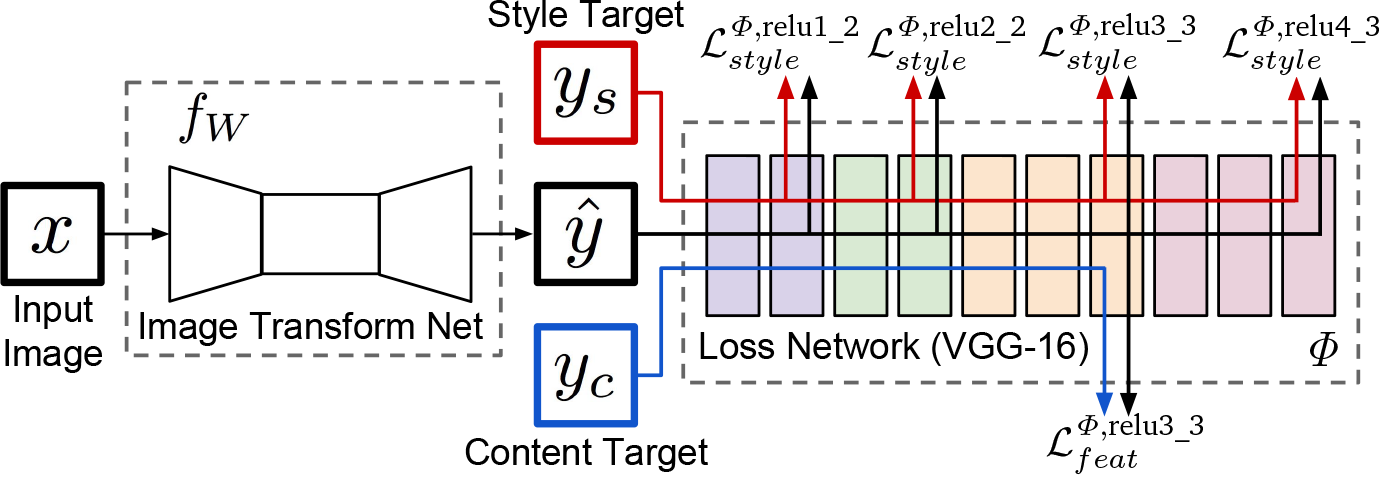
\includegraphics[width=\textwidth]{gfx/app-real-time}
  \caption{
    Overview of \citeauthor{Johnson2016}'s system for image transformation \cite{Johnson2016}.
    The system is composed of an image transformation network $f_W$ and a loss network $\mathit{\Phi}$.
    The image transformation network receives an input image $x$ to produce a transformed image $\hat{y}$.
    The loss network receives the transformed image, a style target $y_s$ and a content target $y_c$ and calculates the feature loss $\mathcal{L}_{feat}$ and the style loss $\mathcal{L}_{style}$ at different stages.
  }
  \label{sec:applications:improvements:real-time}
\end{figure}

The training works by repeating the following process several times.
A content image $x$ is given to the image transformation network and produces a new one $\hat{y}$.
This one is fed to the loss network with the style source $y_s$ we want the network to learn, and the original content image as $y_c$.
The loss network calculates the the feature loss $\mathcal{L}_{feat}$ as well as the style loss $\mathcal{L}_{style}$ and they are used as the loss function for adjusting the weights of the transformation network.
Like this, the image transformation network effectively learns how to transfer a particular style onto given content images in a simple feedforward pass.

\paragraph{Perceptual Quality}
As highlighted both by \citet{Nikulin2016} and \citet{Yin2016}, Neural Style seamlessly transfers the style only if it is highly repetitive and homogeneous over the whole style image.
Because the style representation is taken over the whole image, the style reconstruction fails to capture local style details like particular face features, or different textures in background and foreground.
In consequence, perceptual quality drops as these details get averaged out when transferred onto the content image.

\citeauthor{Nikulin2016}'s analysis of Neural Style concludes proposing an untested style-content global covariance loss that would potentially result in content-aware style transfer, but they also anticipate its computational infeasibility.

At the same time, \citeauthor{Yin2016} proposes a semi-automatic procedure to ensure content-aware style transfer, as we show in \autoref{sec:applications:improvements:content-aware}.
We can observe a real painting of a hummingbird on a wood board as the style source, and a photograph of a hummingbird on a white background.
The desired result would be making the photograph display the local style properties of the painting on the same local spots.
However, Neural Style produces a washed-out composition of low perceptual quality where the style of the background creeps into the foreground.
The content-aware approach preserves the perceptual details of the photograph while applying the style from the painting.

\begin{figure}[t]
  \captionsetup[subfigure]{labelformat=empty}
  \begin{subfigure}[b]{0.244\textwidth}
    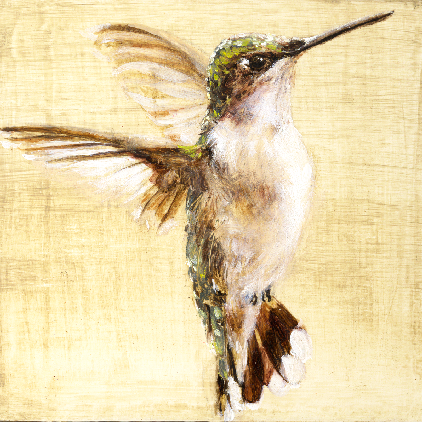
\includegraphics[width=\textwidth]{gfx/app-content-aware-1}
  \end{subfigure}
  \begin{subfigure}[b]{0.244\textwidth}
    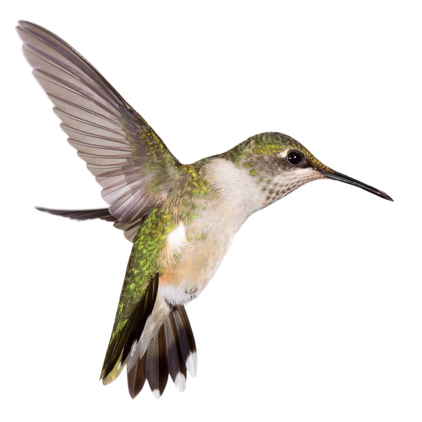
\includegraphics[width=\textwidth]{gfx/app-content-aware-2}
  \end{subfigure}
  \hfill
  \begin{subfigure}[b]{0.244\textwidth}
    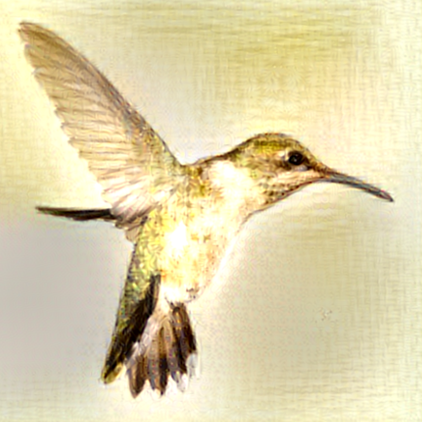
\includegraphics[width=\textwidth]{gfx/app-content-aware-3}
  \end{subfigure}
  \begin{subfigure}[b]{0.244\textwidth}
    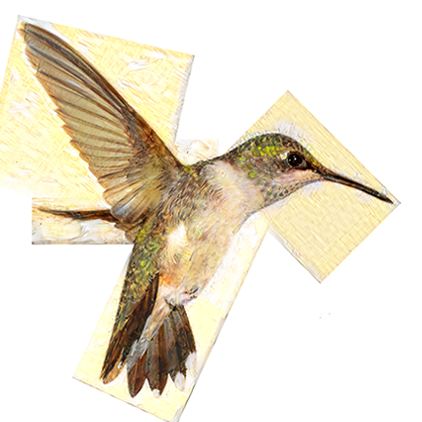
\includegraphics[width=\textwidth]{gfx/app-content-aware-4}
  \end{subfigure}
  \par\smallskip
  \begin{subfigure}[b]{0.244\textwidth}
    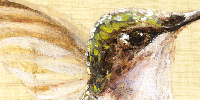
\includegraphics[width=\textwidth]{gfx/app-content-aware-5}
    \caption{Style}
  \end{subfigure}
  \begin{subfigure}[b]{0.244\textwidth}
    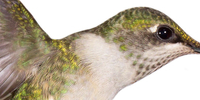
\includegraphics[width=\textwidth]{gfx/app-content-aware-6}
    \caption{Content}
  \end{subfigure}
  \hfill
  \begin{subfigure}[b]{0.244\textwidth}
    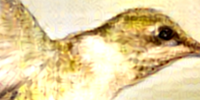
\includegraphics[width=\textwidth]{gfx/app-content-aware-7}
    \caption{Neural Style}
  \end{subfigure}
  \begin{subfigure}[b]{0.244\textwidth}
    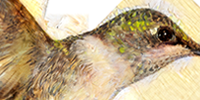
\includegraphics[width=\textwidth]{gfx/app-content-aware-8}
    \caption{Context-Aware}
  \end{subfigure}
  \caption{
    Comparison of Neural Style and content-aware style transfer \cite{Yin2016}.
  }
  \label{sec:applications:improvements:content-aware}
\end{figure}

\citeauthor{Yin2016}'s content-aware procedure consist of the following steps.
First manually segmenting overlapping parts of the foreground content image, being them the head, tail, or wings in this example.
Then, content segments get matched with the local style segments and get processed with the content-aware style transfer algorithm,
The main difference being the content segment is used as the initial image instead of a white noise image.
Lastly, the resulting segments are merged together in the overlapping region.


% ------------------------------------------------------------------------------

\section{Style Transfer Uses}
\label{sec:applications:uses}

Here we present two image transformation tasks inspired by the methods in the Neural Style algorithm.
One of them simply applies style transfer to videos, while the other uses the perceptual loss proposed by \citeauthor{Gatys2015B} for super-resolution.

\paragraph{Neural Style Video}
The first obvious extension of Neural Style is applying it on the different frames of a video to obtain an stylized version of the original one.
But one of the problems with the naive approach of transferring the style to each frame of the video independently is that it results in notable flickering.
This occurs due to Neural Style being initialized with randomly generated white noise image and, therefore, two consecutive frames converge to very different local minima in the optimization process.

\citet{Ruder2016} proposes a system that prevents, among other artifacts, flickering by introducing a temporal constraint that penalizes deviations between consecutive frames, and produces smooth transitions.
\autoref{sec:applications:uses:video} compares the results of processing frames of a video independently and with their system, best observed in the video they provide at \url{https://youtu.be/vQk_Sfl7kSc}.
On it, we can appreciate how the colors are randomly generated for each frame when processed independently, whereas with their system the foreground and background maintain coherent colors throughout the video.

\begin{figure}[t]
  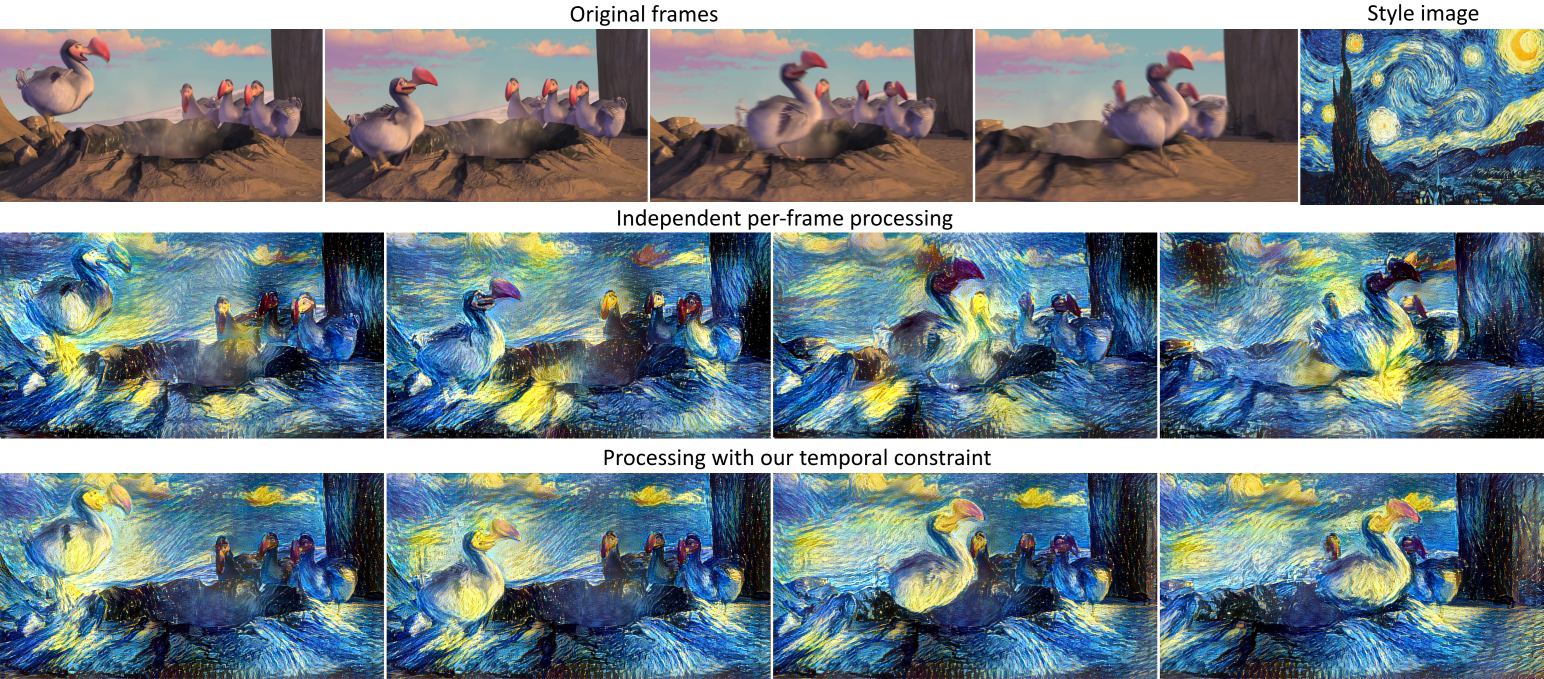
\includegraphics[width=\textwidth]{gfx/app-neural-video}
  \caption{
    Scene from Ice Age (2002) processed in the style of The Starry Night \cite{Ruder2016}.
    Comparison of independent per-frame style transfer to the time constraint approach.
    Comparing independent per-frame processing to the time consistent approach.
    Flicker can be appreciated in the former as the colors of the dodo change frame to frame.
  }
  \label{sec:applications:uses:video}
\end{figure}

\citeauthor{Ruder2016}'s system solve flickering by initializing the style transfer algorithm for a given frame with the previous stylized frame.
This alone achieves that, during the loss optimization process, unchanged areas are found already optimized and do not need to change, while the rest of the frame gets rebuilt.
The method can be made robust against scenes with motion by calculating the optical flow of the frame and warping the pixels of the stylized frame in that direction before feeding it to the style transfer algorithm as the initial image.
Lastly, they include an explicit per-pixel temporal consistency loss to encourage stronger consistency between consecutive frames during the optimization process.

\paragraph{Super-resolution}
As we mentioned before, \citeauthor{Johnson2016}'s architecture for learning style transfer enables it for other image transformation tasks, and super-resolution is one of them.
Super-resolution goal is, given a low resolution image, to produce a larger resolution version.
Recent methods typically train convolutional neural networks using a per-pixel loss between the output and ground-truth images \cite{Dong2016}.
Instead, \citeauthor{Johnson2016}'s image transformation network can learn how to apply super-resolution using high-level features by using the perceptual content loss used in Neural Style, producing more compelling details than the estate of the art.

Like in style transfer tasks, there is no single correct output, as there are many high-resolution images that could have generated the same low-resolution input, and, therefore, semantic reasoning helps producing features that are more visually meaningful to humans.
By using the VGG-16 pre-trained for object recognition as the loss network, the image transformation network is capable of inferring fine details from the visually ambiguous low-resolution inputs.

\autoref{sec:applications:uses:super-res} depicts a super-resolution task comparing per-pixel loss and feature loss.
We can observe how bicubic interpolation, a simple mathematical operation, produces very blurry results.
Comparatively, state-of-the-art deep neural network approach minimizing per-pixel loss $\mathcal{L}_{pixel}$, although objectively superior to the other approaches, does not a yield more compelling result.
Lastly, \citeauthor{Johnson2016}'s approach recreates fine details, as we can clearly see the horses' legs and their hooves.

\begin{figure}[t]
  \begin{subfigure}[b]{0.244\textwidth}
    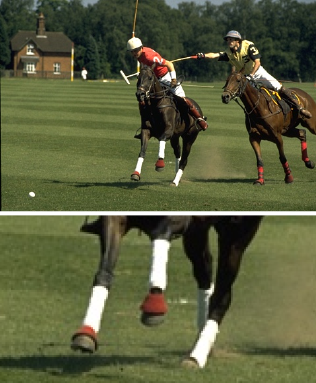
\includegraphics[width=\textwidth]{gfx/app-super-res-1}
    \caption{Ground Truth}
  \end{subfigure}
  \begin{subfigure}[b]{0.244\textwidth}
    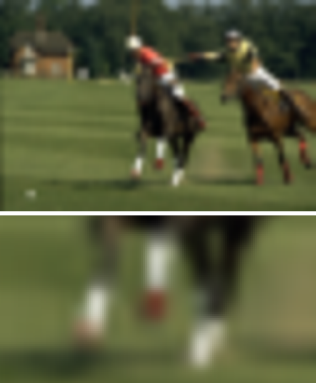
\includegraphics[width=\textwidth]{gfx/app-super-res-2}
    \caption{Bicubic}
  \end{subfigure}
  \hfill
  \begin{subfigure}[b]{0.244\textwidth}
    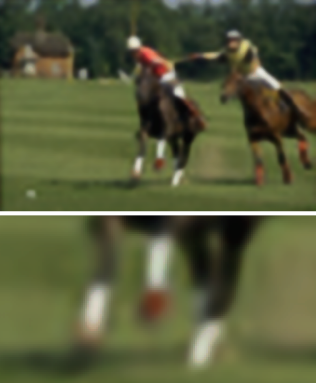
\includegraphics[width=\textwidth]{gfx/app-super-res-3}
    \caption{$\mathcal{L}_{pixel}$}
  \end{subfigure}
  \begin{subfigure}[b]{0.244\textwidth}
    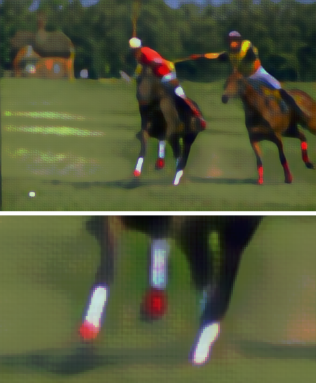
\includegraphics[width=\textwidth]{gfx/app-super-res-4}
    \caption{$\mathcal{L}_{feat}$}
  \end{subfigure}
  \caption{
    Comparison of super-resolution techniques \cite{Johnson2016}.
    Given a low-resolution version of an original image (a), both bicubic method (b) and per-pixel loss function in deep neural networks (c) produce blurry results.
    Using feature loss to train a network for supersampling (d), fine details are inferred.
  }
  \label{sec:applications:uses:super-res}
\end{figure}

If we look again at \autoref{sec:applications:improvements:real-time}, the training process of the image transformation network for a particular super-resolution factor (e.g. $\times{2}$, $\times{4}$, $\times{8}$) works in the following way.
An image $x$, down-sampled accordingly to the factor to be learnt, is given to the image transformation network and produces a new one $\hat{y}$.
The loss network receives the image at the original resolution $y_c$ to calculate the feature loss.
No style loss needs to be calculated in this case, so the loss network calculates the the feature loss $\mathcal{L}_{feat}$ alone.
The image transformation network, minimizing it, effectively learns how to apply super-resolution at the desired factor to given images while maintaining high-level features.


% ------------------------------------------------------------------------------

\section{Beyond Neural Style}
\label{sec:applications:beyond}

Finally, we present another two novel techniques that use deep neural networks to solve perceptive problems: the colorization of grayscale images, and the visual segmentation of concepts in images.

\paragraph{Colorization}
The colorization of grayscale images is also a unconstrained problem, like super-resolution.
Given a grayscale image there are many differently colored versions that could have produced it.
Colorization methods try to generate a set of colors that result believable to a human observer, and, therefore, classic approaches required significant user interaction to provide.

More recently, fully-automatic colorization algorithms have been proposed using deep neural networks and modeling the problem as a regression against per-pixel ground truth colors \cite{Cheng2015}.
The results, however, present desaturated colors.
\citet{Zhang2016} propose a system that approaches the colorization task as a semantic classification problem, relying on perceptual reasoning, and produces vibrant and realistic colorizations, capable of fooling human observers in a color Turing test better than any other method to date.

\autoref{sec:applications:beyond:color} shows a comparison between the regression approach and \citeauthor{Zhang2016}'s classification approach for grayscale colorization.
More examples are available at \url{http://richzhang.github.io/colorization/}.
As we can note, the colors produced by the classification approach do not necessarily match the ground truth, but are more vibrant and believable than those generated through regression.

\begin{figure}[t]
  \captionsetup[subfigure]{labelformat=empty}
  \begin{subfigure}[b]{0.244\textwidth}
    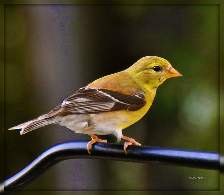
\includegraphics[width=\textwidth]{gfx/app-color-1}
    \caption{Ground Truth}
  \end{subfigure}
  \begin{subfigure}[b]{0.244\textwidth}
    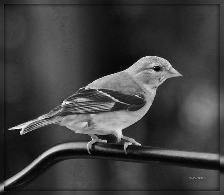
\includegraphics[width=\textwidth]{gfx/app-color-2}
    \caption{Input}
  \end{subfigure}
  \hfill
  \begin{subfigure}[b]{0.244\textwidth}
    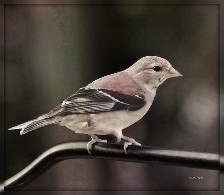
\includegraphics[width=\textwidth]{gfx/app-color-3}
    \caption{Regression}
  \end{subfigure}
  \begin{subfigure}[b]{0.244\textwidth}
    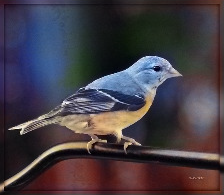
\includegraphics[width=\textwidth]{gfx/app-color-4}
    \caption{Classification}
  \end{subfigure}
  \caption{
    Automatic grayscale image colorization \cite{Zhang2016}.
    Comparison between regression-based and classification-based colorization, the latter producing more vibrant colors.
  }
  \label{sec:applications:beyond:color}
\end{figure}

The system consist in a feedforward pass in a convolutional neural network.
For each pixel of a given grayscale image, a color is inferred based on it semantic classification.
The network, trained over the million color images in ImageNet, is capable of per-pixel class as it has learned the dependencies between the semantics and the textures of grayscale images and their color versions.

Training the network alone did not ensure the generated colors would come out vividly in the generated image.
Caused by non-saturated pixels being orders or magnitude more abundant than saturated ones in ImageNet, the network is more likely to propose the former.
This asymmetry is expected, as image backgrounds tend to be in the spectrum of non-saturated colors, and, therefore, color probabilities are normalized to incentivize foreground, more saturated colors.

Finally, \citeauthor{Zhang2016}'s network can produce more vibrant colors compared to prior attempts thanks to quantizing the color space in buckets.
The Euclidean distance is generally used to measure the loss between a generated image and its ground truth.
This, however, favors gray tonalities.
For instance, if an object can be red or green (e.g. an apple), the ``correct'' color using the Euclidean distance should fall in between, but would never be the pure red nor the pure green.
Instead, by using color buckets, when the predicted color falls in the bucket of the red color space the Euclidean distance is simply measured with respect to the correct tonality of red, not being affected at all by the possibility of green also being a correct color.

\paragraph{Semantic Segmentation}
Image semantic segmentation is the task of partitioning an image into coherent sections.
Traditionally, this was done without actually understanding the semantics of the image, rather by using handcrafted features like color or brightness variations.

\begin{figure}[t]
  \captionsetup[subfigure]{labelformat=empty}
  \begin{subfigure}[b]{0.244\textwidth}
    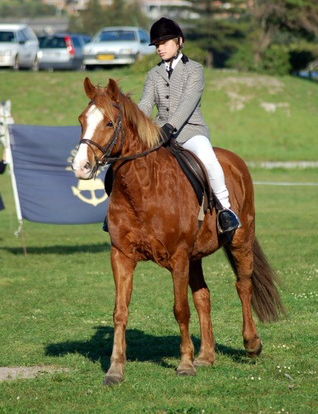
\includegraphics[width=\textwidth]{gfx/app-segmentation-1}
    \caption{Image}
  \end{subfigure}
  \begin{subfigure}[b]{0.244\textwidth}
    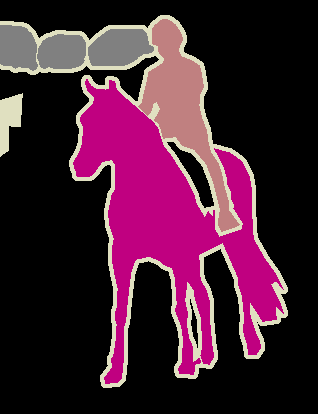
\includegraphics[width=\textwidth]{gfx/app-segmentation-2}
    \caption{Ground Truth}
  \end{subfigure}
  \hfill
  \begin{subfigure}[b]{0.244\textwidth}
    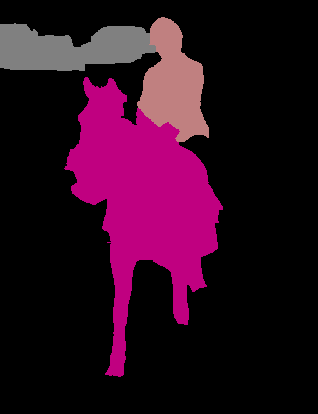
\includegraphics[width=\textwidth]{gfx/app-segmentation-3}
    \caption{SDS \cite{Hariharan2014}}
  \end{subfigure}
  \begin{subfigure}[b]{0.244\textwidth}
    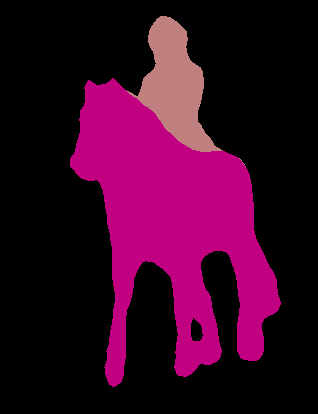
\includegraphics[width=\textwidth]{gfx/app-segmentation-4}
    \caption{FCN \cite{Long2015}}
  \end{subfigure}
  \caption{
    Semantic segmentation \cite{Long2015}.
    Comparison between ground truth, Simultaneous Detection Segmentation and Fully Convolutional Segmentation results.
  }
  \label{fig:sec:applications:beyond:segmentation}
\end{figure}

Convolutional neural networks have been used for per-pixel classification \cite{Farabet2013,Hariharan2014}, but did not generalize well, as they required pre- and post- processing.
\citet{Long2015} proposes a fully convolutional network for semantic segmentation that adapts contemporary classification networks to transfer their learned representations, does not require pre- nor post-processing, is more efficient, and exceeds state-of-the-art performance.

\autoref{fig:sec:applications:beyond:segmentation} shows \citeauthor{Long2015}'s fully-convolutional segmentation (FCN) results compared with the previous state of the art Simultaneous Detection Segmentation (SDS) \cite{Hariharan2014}.
We can see how the whole shape of the horse with its rider was recovered, and how even fine structures like the legs are intact.

\citeauthor{Long2015} system can be implemented converting any convolutional networks pre-trained for object recognition into a fully-convolutional network, followed by fine-tuning it for semantic segmentation.
By converting the convolution network, with fully-connected layers, into a fully-convolutional, without fully-connected layers, they effectively make it learn pixel-wise transformation end-to-end in the fine-tuning step.

The fine-tuning consists in re-training the later layers of the network, more relevant to the task at hand, without discarding the learned weights in the lower layers, more generic.
In this case, the pre-trained network gets trained for semantic segmentation using the PASCAL VOC 2011 training dataset, with ground truth for segmentation tasks and effectively teaching to produce the per-pixel predictions we can see in \autoref{fig:sec:applications:beyond:segmentation}.
